\chapter{Advanced platform administration}\label{chap:PlatformAdministration}

%==================================================================
%================== PRIMERA SECCI�N ===============================
%==================================================================


%%\section{Custom Installation } \label{sec:custom}
%%The custom type installation allows you to select or un-selecting individually packages to be install in the system. 
%%If any of the following software have been installed in the system \footnote{ The installation of any of these software components can cause conflicts in the system if already they exists.}, it is necessary to unselect these packages for installation. Once the installation process finished, the instructions cited here per each particular software must be followed.
%%\begin{itemize}
%%\item \textbf{MySQL}

%%In order to work correctly with \textsc{Thomas}, it is necessary to add a new user called ``thomas'' and to create the \textsc{Thomas} schema in the MySQL database. The following command must be executed:

%%\begin{verbatim}
%%$ cd ~/Magentix2/bin/MySQL
%%$ sh Import-ThomasDB.sh [MYSQL_ROOT_PASS]
%%\end{verbatim}

%%This command creates:
%%\begin{itemize}
%% \item User ``thomas'' with password ``thomas''.
%%\item \textsc{Thomas} schema. This contains all database tables and relationships needed for the \textsc{Thomas} system.
%%\end{itemize}

%%\item  \textbf{Apache Tomcat}
%%To configure Apache Tomcat to work properly with Magentix2, it is needed to move the content from the \textsc{Thomas} directory to the current \textit{webapps/} tomcat directory:

%%\begin{verbatim}
%%$ cd ~/Magentix2/thomas
%%$ mv * /tomcat_directory/webapps
%%\end{verbatim}

%%\item \textbf{Apache Qpid}

%%The broker Qpid must be running in the system in order to connect agents:
%%\begin{verbatim}
%%$ cd $QPID_INSTALLATION
%%$ sbin/qpidd
%%\end{verbatim}


%%\end{itemize}

%%On the other hand, if any of these components  were installed during the Magentix2 Desktop version installation, they would be configured as follows:
%%\begin{itemize}
%%\item \textbf{MySQL:}
%%	it would be installed in the directory \emph{mysql/}.

%%	By default, mysql root password is \textbf{mypassword}, this can be change in any moment.
%%\item \textbf{Apache Tomcat:}
%%	it would be installed in the directory \emph{apache-tomcat-7.0.4/} and 
%%	\textbf{8080} is the port configured to receive services petitions.

%%	The Catalina.out is a log for tomcat, it can be found in log tomcat directory.
%%\item  \textbf{Apache Qpid:}
  %%    it would be installed in the directory \emph{/opt/qpid/} and
    %%  \textbf{5672 } is the port configured to receive connections.

%%\end{itemize}



%%\subsection{Magentix2 installation description}

%%The following folders are created in the selected installation directory (by default \textit{\~{}/Magentix2}) both when full or  custom installation mode is selected ( depending on the selected packages):

%%\begin{itemize}
%%\item \textbf{bin/} 
 %%includes the executable files and folders required to launch and start the platform and services.
 %% These are:
%%\begin{itemize}
 %%\item \textit{Start-Magentix.sh}: it launches services and base agents of the platform \footnote{Magentix2 is launched without security, to enabled security refer to section \ref{sec:DesktopWithSecurity}}. Execute this script is not necessary the first time,  because the installer program do it. 
%%\item \textit{Stop-Magentix.sh}: it stops services and agents of the platform.
%%\item \textit{Launch-MagentixAgents.sh}: it launches the Magentix2 base agents (OMS, SF, TM and bridge agents).
%%\item \textit{Stop-MagentixAgents.sh}: it stops the Magentix2 base agents.
%%\end{itemize}
%%This services can be managed separately, existing a subdirectory per each service.

%%\begin{itemize}
%%\item \textbf{MySQL/} start, stop and configure MySQL service scripts.
%%\item \textbf{Tomcat/} start and stop Apache Tomcat service scripts.
%%\item \textbf{Qpid/} start and stop Apache Qpid service.
%%\end{itemize}



 
%%\textbf{Note:} All the commands could been executed as follows:
%%\begin{verbatim}
%%$ cd  ~/Magentix2/bin or ~/Magentix2/bin/subdirectory
%%$ sh script_name.sh
%%\end{verbatim}

%%In addition, also the following sub-directories are included:
%%\begin{itemize}
 
%%\item \textbf{configuration/} sub-directory: includes the Settings.xml and loggin.xml configuration files, necessary to launch Magentix2 user agents.

%%\item \textbf{security/} sub-directory: includes all required files to launch Magentix2 in secure mode. 
 
%%\end{itemize}


%%\item \textbf{docs/}
 %%includes javadoc and the Magentix2 documentation in Pdf format.
%%\item \textbf{lib/}
 %%includes Magentix2 library an all additional libraries required by Magentix2. How to import this library in projects is explained in  section \ref{sec:devel1stAgent}.
%%\item \textbf{examples/}
 %%includes some examples of Magentix2 agents implementation.
%%\item \textbf{src/}
 %%includes Magentix2 sources.
%%\item \textbf{thomas/}
%% includes all services required by \textsc{Thomas} and Magentix2 platform. It also includes an example of a user web service.
%%\end{itemize}
 





%%\subsection{Possible Errors}

%%If MySQL is already installed in system,  the system informs about it with this error message:

%%\begin{codigo}
 %%   101124 16:20:15 mysqld_safe Logging to syslog.
%%    101124 16:20:16 mysqld_safe A mysqld process already exists
  %%  bin/mysqladmin: connect to server at 'localhost' failed
%%\end{codigo}

%%Moreover, if the following log is showed and \textsc{/etc/mysql/} directory \footnote{If it exists, it is recommended to delete it.} not exists, then an unstable installation of MySQL is in system. In this case,   a new installation of MySQL is recommended.
%%In section \ref{sec:MySQL} is explained how to install MySQL manually and section \ref{sec:custom} explain how to import the \textsc{Thomas} schema in the current MySQL database.

%%\begin{codigo} 
%%    bin/mysqladmin: connect to server at 'localhost' failed
%%    error: 'Can't connect to local MySQL server through 
%%    socket '/tmp/mysql.sock' (2)'
%%    Check that mysqld is running and that the socket: 
%%    '/tmp/mysql.sock' exists!
%%    bin/mysqladmin: connect to server at 'ubuntu' failed

%%    error: 'Lost connection to MySQL server at 'reading initial
%%    communication packet', system error: 111'
 %%   ERROR 2002 (HY000): Can't connect to local MySQL server 
%%    through socket '/tmp/mysql.sock' (2)
%%\end{codigo}

%==================================================================
%================== SEGUNDA SECCI�N ===============================
%==================================================================
\section{Advanced Apache Qpid} \label{sec:apacheQpid}
%Qpid broker is a main component of Magentix2. Probably the contents of this section are not necessary if Magentix2 have been installed  by means of the the desktop version and Qpid was selected to be installed. On the contrary, this section is stronger recommenced in the case it was not desired to install Qpid together with Magentix2, because how to install Qpid  is explained in this section. Apache Qpid can be downloaded from \url{http://qpid.apache.org/download.cgi}
Qpid broker is a main component of Magentix2. In this section is described how it can be installed, in case it was not desired to install Qpid together with Magentix2. Apache Qpid can be downloaded from \url{http://qpid.apache.org/download.cgi}


The   following   libraries   must   be   installed   before   building   the   source distribution of Qpid:
\begin{itemize}
\item libboost�iostreams 1.35�dev: \url{http://www.boost.org} (1.35)
\item  e2fsprogs: \url{http://e2fsprogs.sourceforge.net/} (1.39)
\item pkgconfig: \url{http://pkgconfig.freedesktop.org/wiki/} (0.21)
\item uuid 1.2�1.41.4
\item ruby 4.2
\item ruby 1.8
\end{itemize}
In Ubuntu operating systems these packages can be installed using the Synaptic package management tool, but any other package manager might be valid. As an example, figure \ref{img:qpid1} shows how to install the libboost-iostreams 1.35-dev library. 
\begin{figure}
\centering
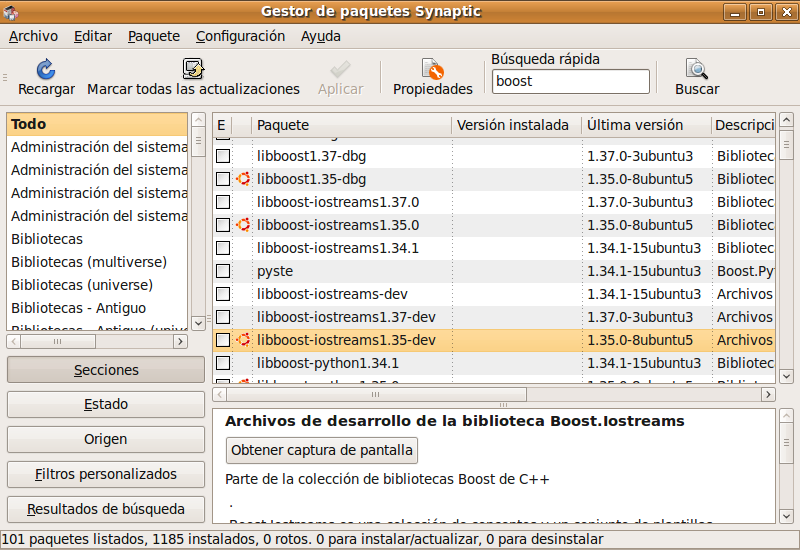
\includegraphics[scale=0.45]{Administration/images/qpid1}
\caption{Installing libboost-iostreams 1.35-dev library with Synaptic tool}
\label{img:qpid1}
\end{figure}
Once all the required libraries have been installed, Qpid broker can be downloaded from: \url{http://qpid.apache.org/download.cgi}. To install Qpid the following steps must be performed: %\footnote{ To install a Qpid version with security support, please follow at this section \ref{sec:QpidWithSecurity}}
\begin{itemize}
 \item Uncompressing the donwloaded Qpid file.
 \item  \texttt{\$ ./configure --prefix= /opt/qpid} $\rightarrow$ Using the prefix  option when configuring, the location where the Qpid binaries are installed can be specified (in this example case, /opt/qpid).
 \item \texttt{\$ make install}
\end{itemize}

After a successful installation Qpid can be launched executing the following command inside the folder where Qpid was installed (in this example case, /opt/qpid): \texttt{\$ ./qpidd}.

Some values Qpid broker set by default are used by some components of Magentix2, therefore if any of them is changed, it is possible that the Settings.xml file has to be also modified. This file can be found in the configuration directory of Magentix2 distribution folder. Specifically the parameters that affect Qpid configuration in the Settings.xml file are the following:
\begin{codigo}
<entry key="host">localhost</entry>
<entry key="port">5672</entry>
<entry key="vhost">test</entry>
<entry key="user">guest</entry>
<entry key="pass">guest</entry>
<entry key="ssl">false</entry>
\end{codigo}

For example, if the port which Qpid broker is listening to is modified from the default 5672 to 5671, this change has to be also made on the Settings.xml file.

For those looking to adjust the Qpid broker operation there are plenty of advanced configuration options, for further information, please, refer to: \url{http://qpid.apache.org/books/0.7/AMQP-Messaging-Broker-CPP-Book/html/index.html}. Please note that if two ore more Qpid brokers have to work federated, a link between all the broker's amq.topic exchange has to be added.

%==================================================================
%================== TERCERA SECCION ===============================
%==================================================================
\section{Advanced MySQL}\label{sec:MySQL}
MySQL is a main component of the \textsc{Thomas} framework. This section explains how to properly configure MySQL to work in conjunction with \textsc{Thomas}. This section helps you to configure MySQL properly.


All   the   information   about   the  organizations  created with the \textsc{Thomas} framework and running on the Magentix2 platform  
is  permanently  stored   in a MySQL database. It is possible to create the  database schema and the user  employed by the \textsc{Thomas} framework  in MySQL by means of the the execution of the script \textit{magentix-setup.py}. This script is located in the main directory of  the Magentix2 installation folder. The commands needed to execute this script are the following (from the Magentix2 root directory):


\begin{verbatim}
$ python magentix-setup.py
\end{verbatim}

However, it is also possible to create the \textsc{Thomas} database infrastructure step by step, without using the cited script. In this case, it is necessary to load into MySQL the   complete   structure   of   the   database from the \textit{db-schema.sql} and \textit{grants.sql} files. These files are located into the directory  \verb|bin/sql/|. In order to load these files,  the \textit{MySQL Administrator} tool should be opened,  and then  the \textit{Restore Backup} option must be selected, choosing the \textit{db-schema.sql} backup file to be restored. An example of this procedure can be shown in the figure \ref{img:mysql1}

\begin{figure}[!h]
\centering
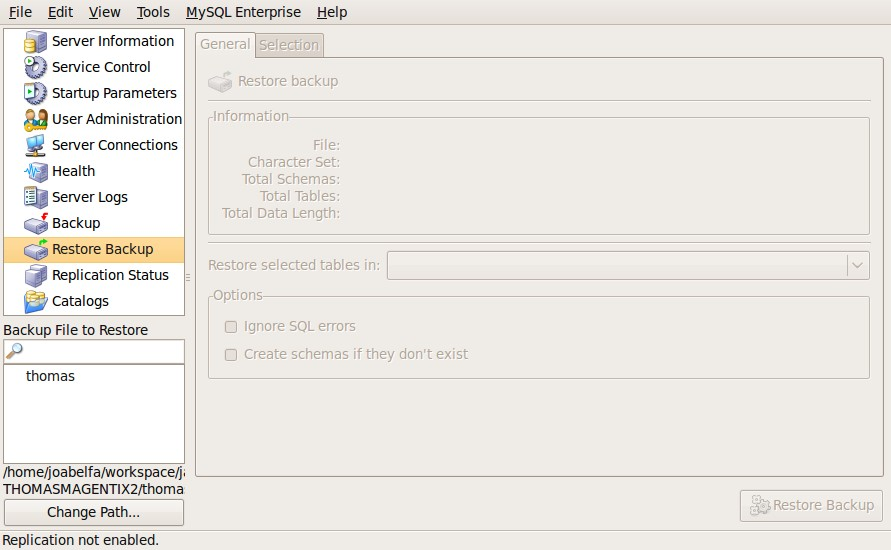
\includegraphics[scale=0.45]{Administration/images/mysql1}
\caption{Restoring the \textit{db-schema.sql} backup file in the \textit{Restore Backup} option of the \textit{MySQL Administrator}}  
\label{img:mysql1}
\end{figure}

The next required step is to add a new user to the \textsc{Thomas} schema in the \textit{User Administration} option of the \textit{MySQL Administrator} tool (see Figure \ref{img:mysql2}). The required fields must be fulfilled with the following information:

\begin{verbatim}
User=thomas
Password=thomas
\end{verbatim}

You can automate this step by loading the \textit{grants.sql} file.

\begin{figure}[!h]
\centering
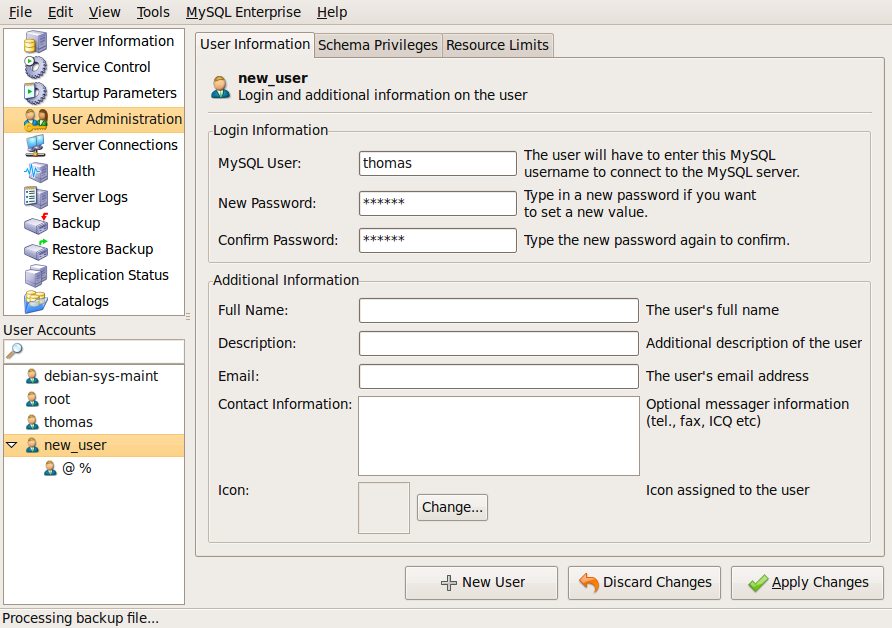
\includegraphics[scale=0.45]{Administration/images/mysql2}
\caption{Adding the necessary user information into the \textsc{Thomas} schema in the \textit{User Administrator} option of the \textit{MySQL Administrator} tool}
\label{img:mysql2}
\end{figure}

The \textit{ServerName}, \textit{databaseName}, \textit{userName} and \textit{password} entries must be also configured in the Settings.xml file located in the \verb|configuration/| directory.
The parameters that affect MySQL configuration in the Settings.xml file are the following:

\begin{codigo}
<!-- Properties mysql -->
<entry key="serverName">localhost</entry>
<entry key="databaseName">thomas</entry>
<entry key="userName">thomas</entry>
<entry key="password">thomas</entry>
\end{codigo}

On the other hand, the THOMAS framework uses Apache Jena for manage the semantic description of the services.
In order to specify the required parameters for Jena, the Settings.xml file located in the \verb|configuration/| directory
will be configured. The parameters that affect Jena configuration in the Settings.xml file are the following:
\begin{codigo}
<!-- Properties jena -->
<entry key="dbURL">jdbc:mysql://localhost/thomas</entry>
<entry key="dbType">MySQL</entry>
<entry key="dbDriver">com.mysql.jdbc.Driver</entry>
\end{codigo}

Check if the direction where agents OMS and SF are running is different host from where the MySQL is configured with the data base schema employed by the THOMAS framework.
If the OMS and SF are running in the same host, the configuration by default is correctly.

Finally, all available privileges for \textsc{Thomas} tables must be assigned to the \textit{thomas} user (Figure \ref{img:mysql4})
\begin{figure}[th!]
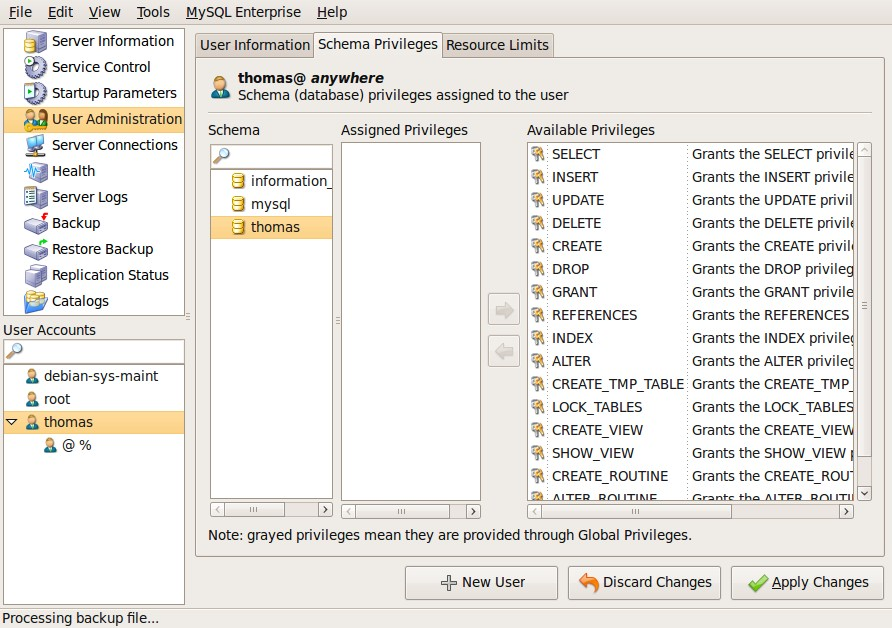
\includegraphics[scale=0.45]{Administration/images/mysql4}
\caption{Assigning privileges to the \textit{thomas} user in the \textit{User Administration} option of the \textit{MySQL Administration tool} }
\label{img:mysql4}
\end{figure}

%==================================================================
%================== CUARTA SECCI�N ================================
%==================================================================
\section{Advanced Apache Tomcat}
Apache Tomcat is a main component of Magentix2, because it allows to access to standard Java web services. If Apache Tomcat was installed during the Magentix2 Desktop version installation,  it will not be necessary to follow the steps shown here. On the other hand, this section helps to configure it properly.

\textsc{Thomas}   platform   is   based   on   services (chapter \ref{chap:VirtualOrganizations}),   so   SF   and   OMS   service implementations have to be available as standard web services. Moreover, Magentix2 offers another service named MMS ( section \ref{sec:security}), which is responsible of controlling the user access to the platform.  This service must be also available as an standard web service. Any other user service (such as the application examples) need also to be available as standard web services. As mentioned above, Magentix2 uses Apache Tomcat to allow it. 


Apache Tomcat can be downloaded from: \url{http://tomcat.apache.org/}. The installation instructions can be found at: \url{http://tomcat.apache.org/tomcat-7.0-doc/setup.html}.

Once Tomcat is installed, packaged libraries of \textsc{Thomas} services (omsservices.war, sfservices.war)  have to be copied from the \verb|webapps/| directory of the Magentix2 installation to the subdirectory\\ \verb|webapss/| of the Tomcat installation directory. %%Furthermore, the packaged library of the MMS service (MMS.war), which is also located at the  \verb|Magentix2/thomas/| directory, must  be  copied to the same \verb|webapss/|  subdirectory.

Then, the path where web services are deployed is required. In order to specify these parameters, the Settings.xml file
located in the configuration/ directory will be configured
The parameters that affect THOMAS configuration in the Settings.xml file are the following:
\begin{codigo}
<!-- Properties thomas -->
<entry key="OMSServiceDescriptionLocation">
	http://localhost:8080/omsservices/services/
</entry>
<entry key="SFServiceDescriptionLocation">
	http://localhost:8080/sfservices/services/
</entry>
\end{codigo}

Check if the direction where agents OMS and SF are running is different host from where the services (OMS and SF) are deployed, or if the port is different.
If the OMS and SF are running in the same host that  web services are deployed, the configuration by default is correctly.

In the same way, in order to run any developed web service from Tomcat, it is necessary to copy the packaged library (serviceName.war) to the subdirectory \verb|webapss/| of the Tomcat installation directory. %%In Magentix2 there is an example of a user web service, called \textit{SearCheapHotel}. It is possible to run this  example by means of coping the packaged library SearchCheapHotel.war (located at the \verb|Magentix2/thomas/| directory) to the subdirectory \verb|webapss/|  of Tomcat 



Once all the necessary services have been properly copied to the webapss directory, Tomcat can be started running the startup.sh file on the \verb|/bin/| subdirectory of the Tomcat installation directory.




\begin{figure}[!h]
\centering
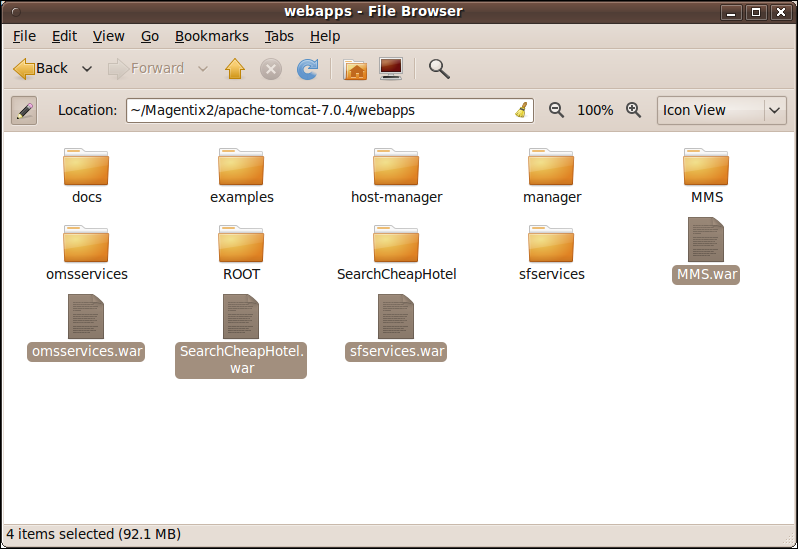
\includegraphics[scale=0.45]{Administration/images/tomcat1.png}
\caption{Location of web services files (*.war)}
\label{img:tomcat1}
\end{figure}



%==================================================================
%================== QUINTA SECCI�N ================================
%==================================================================
\section{Advanced platform services}
This section explains how to launch platform agents without using the standard methods shown previously on this manual. This can be useful when some default parameters have been changed or if the platform runs in a distributed way.
\subsection{Running Bridge Agents}\label{sec:AdminRunningBridgeAgents}

Bridge agents are in charge of sending and receiving messages to or from foreign agents. For example, they allow Magentix2 agents to communicate with Jade agents. \textit{BridgeAgentInOut} manages messages that go from inside the platform to outside, whereas \textit{BridgeAgentOutIn} does the opposite. Bridge agents can be running on any host, they do not have to be in the same host where the QPid broker or other agents are running. A Java program has to be written and executed in order to launch bridge agents. The following code shows how to launch these agents:
\begin{lstlisting}
import es.upv.dsic.gti_ia.core.AgentsConnection;
import es.upv.dsic.gti_ia.core.AgentID;
import es.upv.dsic.gti_ia.core.BridgeAgentInOut;
import es.upv.dsic.gti_ia.core.BridgeAgentOutIn;

public class Main {
   public static void main(String[] args) throws Exception {
      AgentsConnection.connect();
      private BridgeAgentInOut inOutAgent;
      private BridgeAgentOutIn outInAgent;
      inOutAgent = new BridgeAgentInOut(new AgentID("BridgeAgentInOut"));
      outInAgent = new BridgeAgentOutIn(new AgentID("BridgeAgentOutIn"));
      inOutAgent.start();
      outInAgent.start();
   }
}
\end{lstlisting}
In the code shown above when the bridge agents are created (lines 11-12) they receive a new AgentID as argument. This new AgentID gets only one argument, the name of the agent. Platform agents, like bridge agents, must always have a well known name. For bridge agents the names must be: ``BridgeAgentInOut'' and ``BridgeAgentOutIn'' respectively.

In line 8 the connection of the agents to the platform is set using the method \texttt{AgentsConnection.connect()}. The parameters for this connection are specified in the configuration file \texttt{Settings.xml}. The method \texttt{AgentsConnection.connect()} should not be called if the platform security is enabled.
% 4 arguments, in order:
% \begin{enumerate}
%    \item Agent name: This argument cannot be modified. For the BridgeAgentInOut it must be ``BridgeAgentInOut'' and for BridgeAgentOutIn ``BridgeAgentOutIn''.
%    \item Agent protocol: This argument cannot be modified. For both agents it must be ``qpid''.
%    \item Agent host: Here we specify the ip address of the QPid broker we want to connect the agent to, in this specific example both agents connect to the broker running in the localhost, but we can specify other one, even it is possible to connect each bridge agent to a different QPid broker if these QPid brokers are federated.
%    \item Agent port: This is the port the QPid broker listens to. It has to match the port of the broker the agent connects to.
% \end{enumerate}

Once the agents have been created with the desired parameters, both are started (lines 13 \& 14). This Java program has to be manually executed when starting Magentix2 platform.

\subsection{Running OMS and SF Agents}
OMS and SF agents provide all the services of Thomas framework. These agents can be running on any host, they don't have to be in the same host where the QPid broker or other agents are running. A Java program has to be written and executed in order to launch OMS and SF agents. The following code shows how to launch these agents:

\begin{lstlisting}
import es.upv.dsic.gti_ia.architecture.Monitor;
import es.upv.dsic.gti_ia.core.AgentID;
import es.upv.dsic.gti_ia.core.AgentsConnection;
import es.upv.dsic.gti_ia.organization.OMS;
import es.upv.dsic.gti_ia.organization.SF;
import es.upv.dsic.gti_ia.core.AgentID;

public class Main {
   public static void main(String[] args) throws Exception {
      AgentsConnection.connect();
      OMS agentOMS = OMS.getOMS();
      SF agentSF = SF.getSF();
      agentOMS.start();
      agentSF.start();
   }
}
\end{lstlisting}

In the code shown above the agents OMS and SF are created (lines 11-12). The creation of these agents does not require any parameter.

% In the code shown above when the OMS and SF agents are created (lines 9-10) they receive a new AgentID as argument. This new AgentID gets 4 arguments, in order:

In line 10 the connection of the agents to the platform is set using the method \texttt{AgentsConnec} \texttt{tion.connect()}. The parameters for this connection are specified in the configuration file \texttt{Settings.xml}. The method \texttt{AgentsConnection.connect()} should not be called if the platform security is enabled. 
% 
% \begin{enumerate}
%    \item Agent name: This argument cannot be modified. For the OMS it must be ``OMS'' and for the SF ``SF''.
%    \item Agent protocol: This argument cannot be modified. For both agents it must be ``qpid''.
%    \item Agent host: Here we specify the ip address of the QPid broker we want to connect the agent to, in this specific example both agents connect to the broker running in the localhost, but it can be other one, even it is possible to connect each agent to a different QPid broker, if these QPid brokers are federated.
%    \item Agent port: This is the port the QPid broker listens to. It has to match the port of the broker the agent connects to.
% \end{enumerate}

Once the agents have been created with the desired parameters, both are started (lines 13 \& 14). This Java program has to be manually executed when starting Magentix2 platform.

